%\documentclass[a4paper]{article}

\documentclass[12pt]{article}

%% Language and font encodings
\usepackage[english]{babel}
\usepackage[utf8x]{inputenc}
\usepackage[T1]{fontenc}

%% Sets page size and margins
\usepackage[a4paper,top=3cm,bottom=2cm,left=3cm,right=3cm,marginparwidth=1.75cm]{geometry}

%% Useful packages
\usepackage{amsmath}
\usepackage{graphicx}
\usepackage[colorinlistoftodos]{todonotes}
\usepackage[colorlinks=true, allcolors=blue]{hyperref}

\usepackage{amsfonts} %% for mathbb
\usepackage{verbatim} %% for comment
\usepackage{mathtools} %% aligned equation

\title{The Marginal Value of Adaptive Gradient Methods in Machine Learning}
\author{A. Wilson, R. Roelofs, M. Stern, N. Srebro, B. Recht}

\begin{document}
\maketitle
as understood by Kelly Zhang

\vspace{3mm}
Disclaimer: This presentation is made up of my understandings and intuitions about this paper - as a complete newbie to the land of optimization... Questions and feedback welcome!

Should be fun though!

\section{ \href{https://arxiv.org/pdf/1611.03530.pdf}{Understanding Deep Learning Requires Rethinking Generalization} }
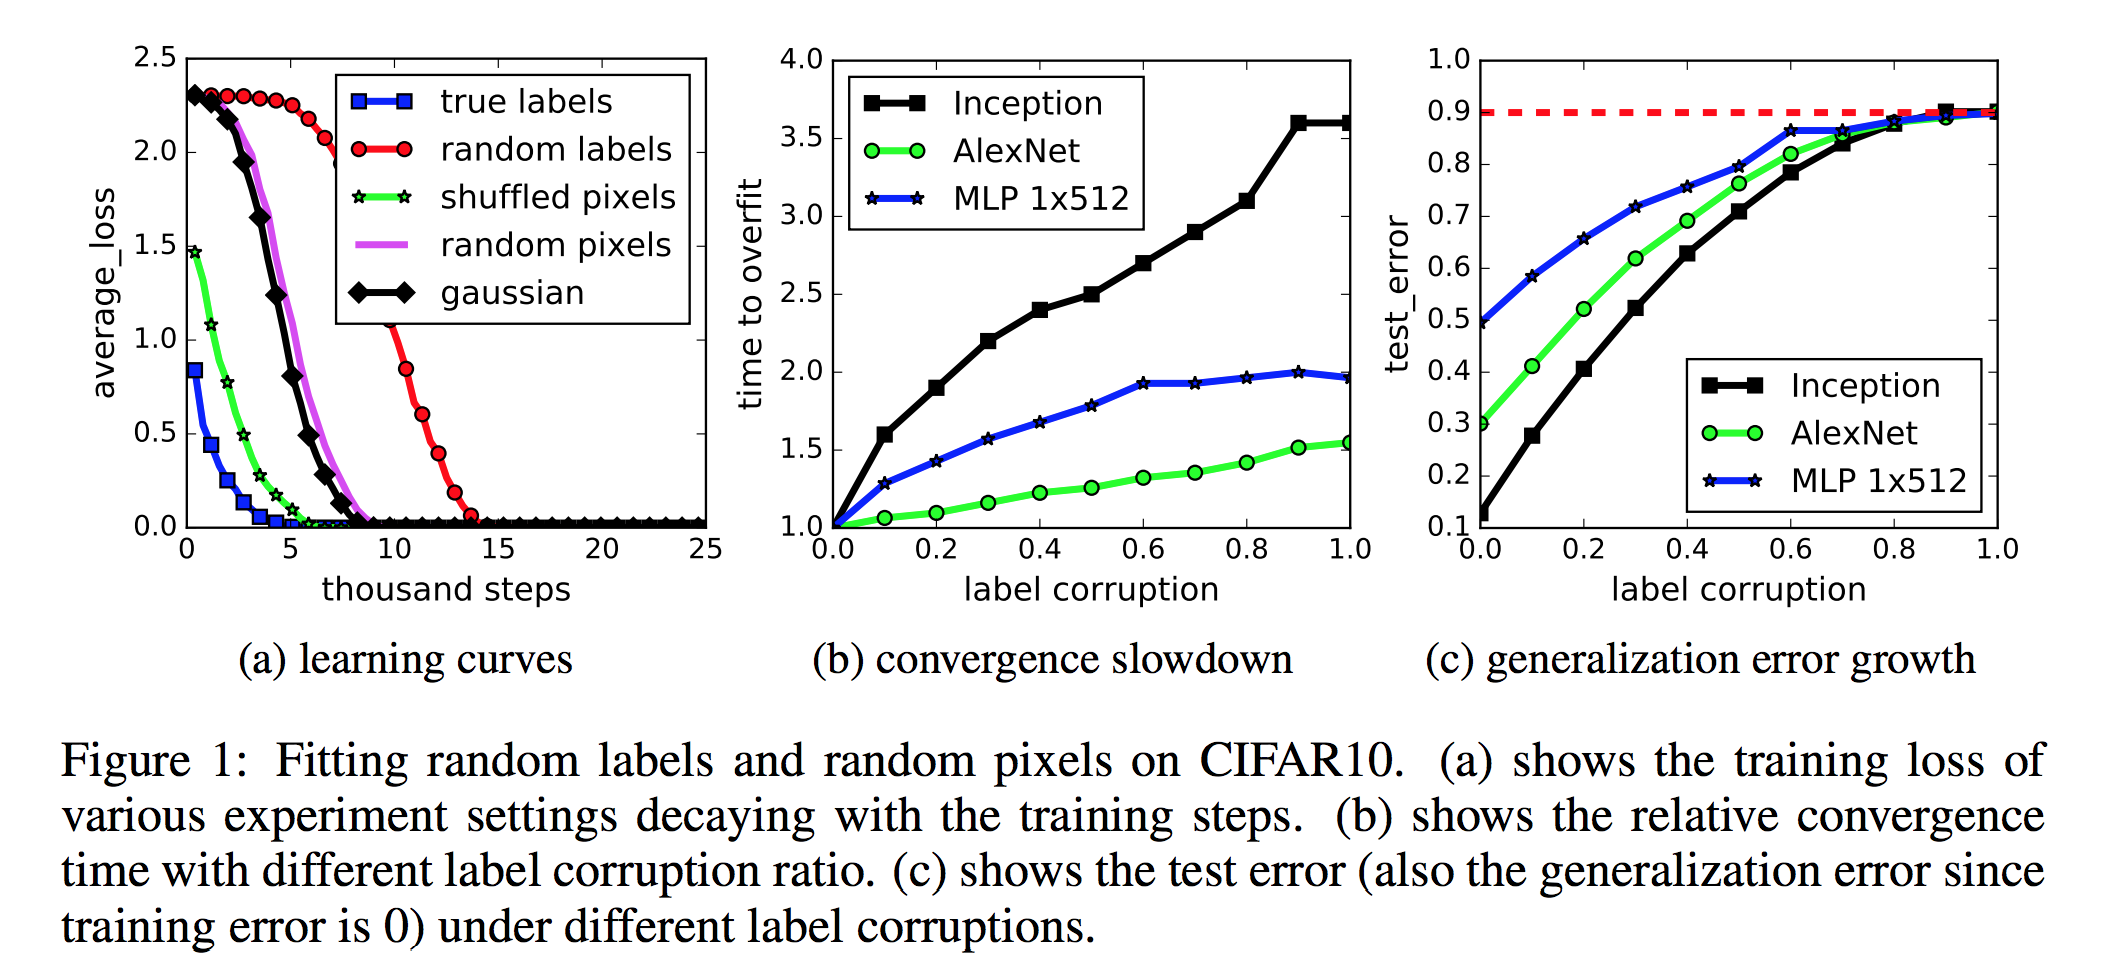
\includegraphics[width=1\textwidth]{rethinking}

\vspace{3mm}

Some relevant takeaways:
\begin{itemize}
	\item The models we're training are over-parametrized, even with regularization (at least for image classification)
	\item Faster convergence does seem to lead to less overfitting / better generalization (similar argument as that for early-stopping as regularization)
\end{itemize}

\newpage
%%%%%%%%%%%%%%%%%%%%%%%%%%%%%%%%%%%%%%%%%%%%%

\section{Generalization in Over-Parameterized Settings}
\begin{itemize}
  \item When models are over-parametrized, there are multiple solutions that minimize training error
  \item Still, some minima can be better than others in terms of generalization
  	\subitem In general, the simplest model that explains the data has better generalization. Thus in the over-parameterized setting, "simplicity" is favored.
	\subitem I am not exactly sure how "simplicity" is measured generally, but we will discuss this in a specific example.
  \item This paper
  	
	1. Proves in a simple model and problem setting where adaptive gradient methods fail to generalize as well as regular SGD (even when both methods achieve zero training error)
	
	2. Empirically shows the inferiority of adaptive gradient methods in terms of generalization on several image and text tasks
\end{itemize}

\begin{comment} %%%%%%%

\subsection{My guess as to "better minima" meaning...}
\todo{MAKE THIS BETTER!!}
Maximizing margin in SVM classifier, which is equivalent to finding minimum norm solution.

The minimum norm solution is the $w$ vector with the minimum L2 norm, which means it separates the data while still being of small norm, meaning it is pointing in a direction of with a large margin of separation.

$$\min_{w} || w ||_2$$
$$s.t. \hspace{5mm} w^T   x^{(i)} \geq \gamma \hspace{8mm} \text{if} \hspace{2mm} y^{(i)} = 1$$
$$\hspace{13mm} w^T   x^{(i)} \leq -\gamma \hspace{5mm} \text{if} \hspace{2mm} y^{(i)} = 0$$

\vspace{5mm}

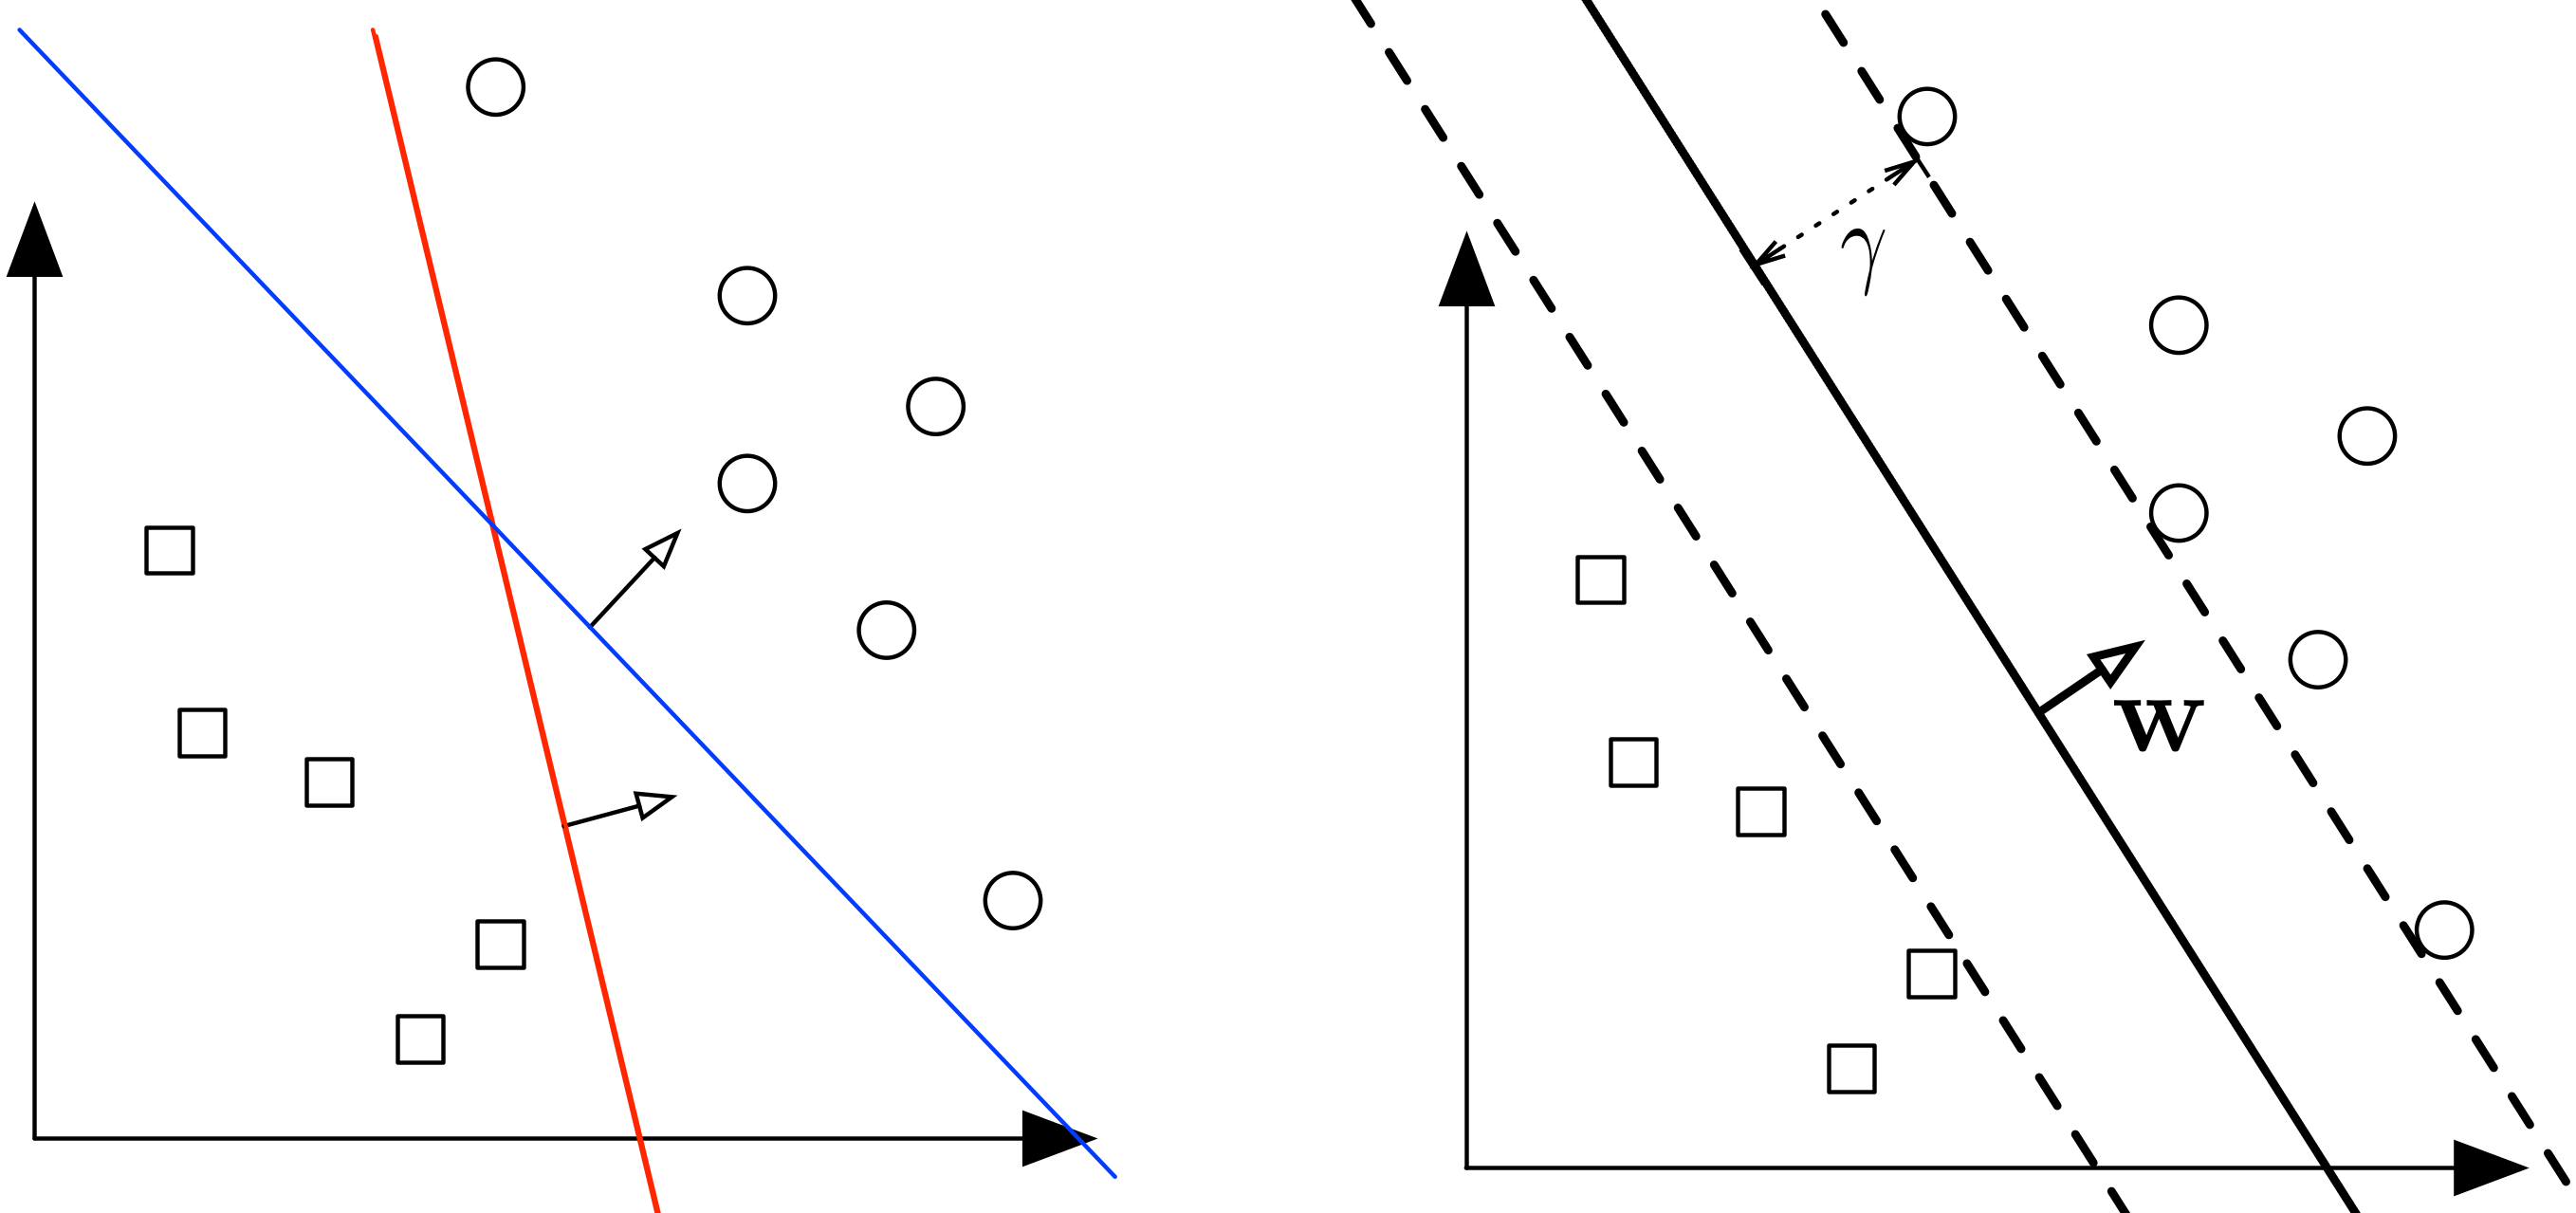
\includegraphics[width=1\textwidth]{svm}

I am still unsatisfied with my current understanding of the concept of finding "better minima" in over-parametrized, under-regularized settings...
\todo{TODO}

\end{comment} %%%%%%%

\vspace{10mm}

\newpage
%%%%%%%%%%%%%%%%%%%%%%%%%%%%%%%%%%%%%%%%%%%%%

\section{Gradient Descent!}

\subsection{SGD}
$$w_{k+1} = w_k - \alpha \tilde{ \nabla } f ( w_k ) $$

where $\alpha$ is the learning rate

\subsection{Momentum}
$$w_{k+1} = w_k - \alpha \tilde{ \nabla } f ( w_k + \gamma_k (w_k - w_{k-1})) + \beta_k (w_k - w_{k-1}) $$

\begin{itemize}
	\item Polyak's heavy-ball method (HB): $\gamma_k = 0$
	\item Nesterov's Accelerated Gradient method (NAG): $\gamma_k = \beta_k$
\end{itemize}

\vspace{5mm}
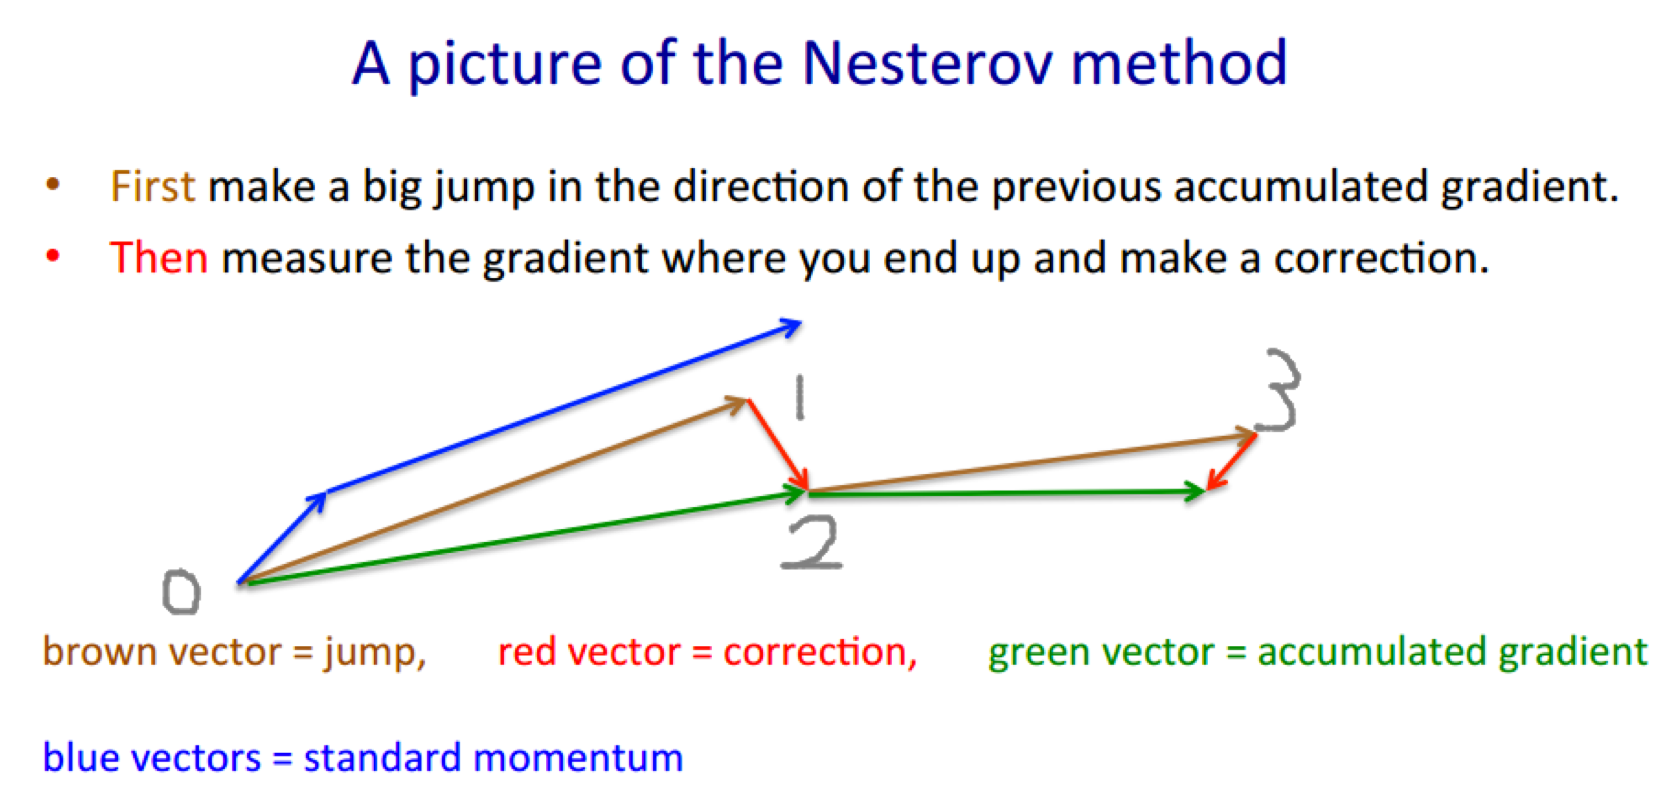
\includegraphics[width=1\textwidth]{nesterov}

\begin{itemize}
	\item Take step in direction of previous gradient: $ \beta_k (w_k - w_{k-1})$
	\item Correction: $w_k - \alpha \tilde{ \nabla } f ( w_k + \gamma_k (w_k - w_{k-1}))$
\end{itemize}

\newpage
%%%%%%%%%%%%%%%%%%%%%%%%%%%%%%%%%%%%%%%%%%%%%

\subsection{Adaptive Gradient Methods}
\textbf{ What are they? How do they relate to each other? }

\subsubsection{Newton's Method}
A procedure way to numerically find the roots or zeros of a function.

%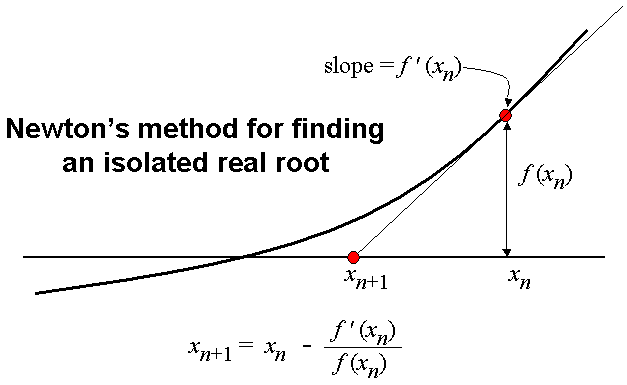
\includegraphics[width=0.5\textwidth]{newton}

\vspace{3mm}
\textbf{Newton's Rule (single variable):}
$$
f(x_{t+1}) = 0 = f(x_t) + f'(x_t) (x_t - x_{t+1})
$$
$$
x_{t+1} = x_t - \dfrac{ f(x_t) }{ f'(x_t) }
$$

Newton's method can easily be adapted to help us find critical points of a function, $g$, by simply setting $f(x) = g'(x)$:
$$
x_{t+1} = x_t - \dfrac{ g'(x_t) }{ g''(x_t) }
$$

\vspace{3mm}
\textbf{Multivariate Newton's method:}
$$w_{k+1} := w_{k} - \alpha H_k^{-1}  \nabla f ( w_k )$$
where $H_k$ is the Hessian of $f( w_k )$.

\vspace{5mm}
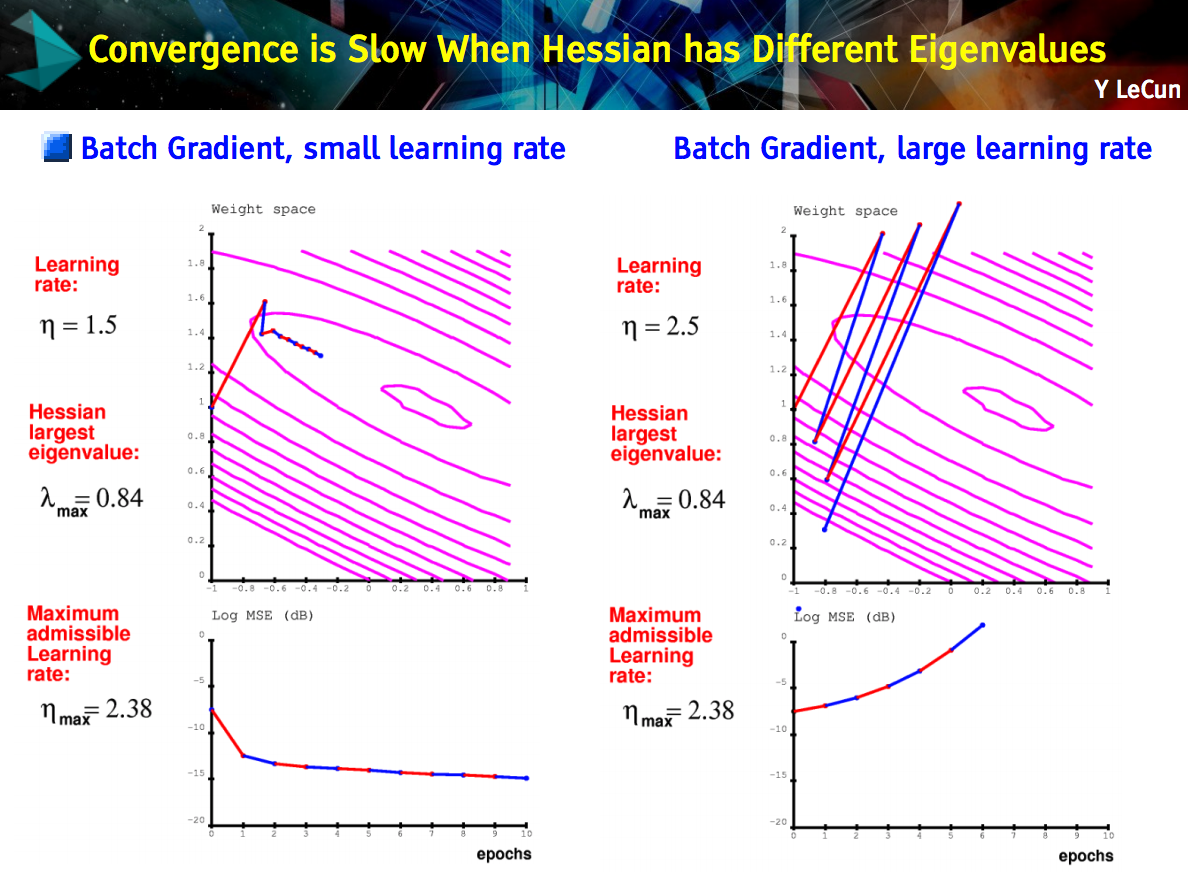
\includegraphics[width=1\textwidth]{hessian}

%Second order method of optimization (rather than approximating function locally with linear function, approximate with quadratic function - extra term in Taylor series). Takes into account the curvature in different directions.


\subsubsection{AdaGrad (by Duchi, Hazan, and Singer, 2011)}
$$w_{k+1} := w_{k} - \alpha H^{ -1}_k \tilde{ \nabla } f ( w_k ) $$
$$G_{k+1} := G_k + D_k$$
$$( H = \sqrt{G} ) $$

Where $D_k$ is a diagonal matrix (with $\tilde{ \nabla } f(w_k)$ squared for each entry):
$$D_k := \text{Diag} \{ \tilde{ \nabla } f(w_k)^2 \}$$
So $G$ is linear combinations of the square of past gradient components.

\vspace{3mm}
\textbf{Note}: 

%From Large Scale Distributed Deep Networks:
%"We conjecture that Adagrad automatically stabilizes volatile parameters in the face of the flurry of asynchronous updates, and naturally adjusts learning rates to the demands of different layers in the deep network."

Different learning rate for each parameter. Larger updates for "infrequent" parameters (small square of gradient over updates) and small updates for "frequent" parameters (large square of gradient over updates).

This feature of adaptive gradient methods is what can lead it give undue influence to "spurious" features.

\subsubsection{RMSProp (by Hinton, unpublished)}
Same as AdaGrad, but with different weighting scheme:

$$w_{k+1} := w_{k} - \alpha H^{ -1}_k \tilde{ \nabla } f ( w_k )$$
$$G_{k+1} := \beta_2 G_k + (1-\beta_2) D_k$$
$$( H = \sqrt{G} ) $$

\subsubsection{ADAM (by Kingma and Ba, 2014)}
$$w_{k+1} := w_{k} - \alpha \hat{H}^{ -1}_{k+1} \hat{g}_{k+1}$$
$$g_{k+1} := \beta_1 g_k + (1 - \beta_1) \tilde{ \nabla } f ( w_k )$$
$$G_{k+1} := \beta_2 G_k +(1 - \beta_2) D_k$$
$$\hat{ g }_{k+1} = \frac{ g_{k+1} }{1 - \beta_1^{k+1}} $$
$$\hat{ G }_{k+1}  = \frac{ G_{k+1} }{ 1 - \beta_2^{k+1} } $$
$$\big( \hat{H} = \sqrt{ \hat{G} } \big) $$

(Note in $\beta_1^k$, $k$ denotes $\beta_2$ to the power $k$.)

\newpage
%%%%%%%%%%%%%%%%%%%%%%%%%%%%%%%%%%%%%%%%%%%%%

\section{Simple Setting for Analysis: Gradient Descent for Linear Regression}

$$\min_w R[w] := || Xw - y ||^2$$
with
\begin{itemize}
	\item $X$ is a $n \times d$ matrix ($n$ for data points; $d$ for features)
	\item $y$ is a $n$-dimensional vector of labels in $\{-1, 1\}$
\end{itemize}

We assume the problem is over-parameterized / over-determined, so $d > n$ (number of features > number of data points).

Thus if there is a $w$ that achieves loss 0, then there are infinitely many global minimizers (solution not unique, since over-complete).

\subsection{Calculating the Gradient}
$$R = (Xw - y)^T (Xw - y) = $$
$$(Xw)^T(Xw-y) - y^T(Xw-y) = $$
$$(Xw)^T(Xw) - (Xw)^Ty - y^T(Xw) + y^Ty$$
$$w^TX^TXw - 2 y^TXw + y^Ty$$
$$w^TX^TXw - 2 (X^Ty)^Tw + y^Ty$$

\vspace{2mm}
Using
$$\frac{d}{dw} y^T w = \frac{d}{dw} w^T y = y$$
$$\frac{d}{dw} w^T X w = (X + X^T) w$$

\vspace{2mm}
We get:
$$\frac{d}{dw} R = (X^TX + XX^T) w - 2X^T y = 2 X^TX w - 2X^T y$$

Thus, $\frac{d}{dw} R \in $ span\{ rows of $X$ \}, since for arbitrary vector $a$, $X^T a$ for is a linear combination of the rows of $X$.

\newpage

\subsection{Non-adaptive methods}
\textbf{Claim}: If $w$ is initialized in the row span of $X$ (e.g. $w = 0$), and uses only linear combination of gradients / stochastic gradients, $w_t$ must also lie in the row span of $X$, for all updates $t$.

\textbf{Justification}: If we start in the span of the rows of $X$, and add linear combinations of the rows of $X$, we will still end up in the span of $X$'s rows.

\vspace{20mm}

\textbf{Claim}:  The unique solution that lies in the row span of X also happens to be the solution with \textbf{minimum Euclidian norm}, so
$$w^{SGD} = X^T (X X^T)^{-1} y$$

\textbf{Justification}: The idea is that since the system is underdetermined, we can think of the problem of finding vector as $w$, as finding the vector in a very high dimensional space, that projects to another vector $y$ in a lower dimensional space (the projection function is determined by $X$). 

$$\min_w R[w] := || Xw - y ||^2$$

%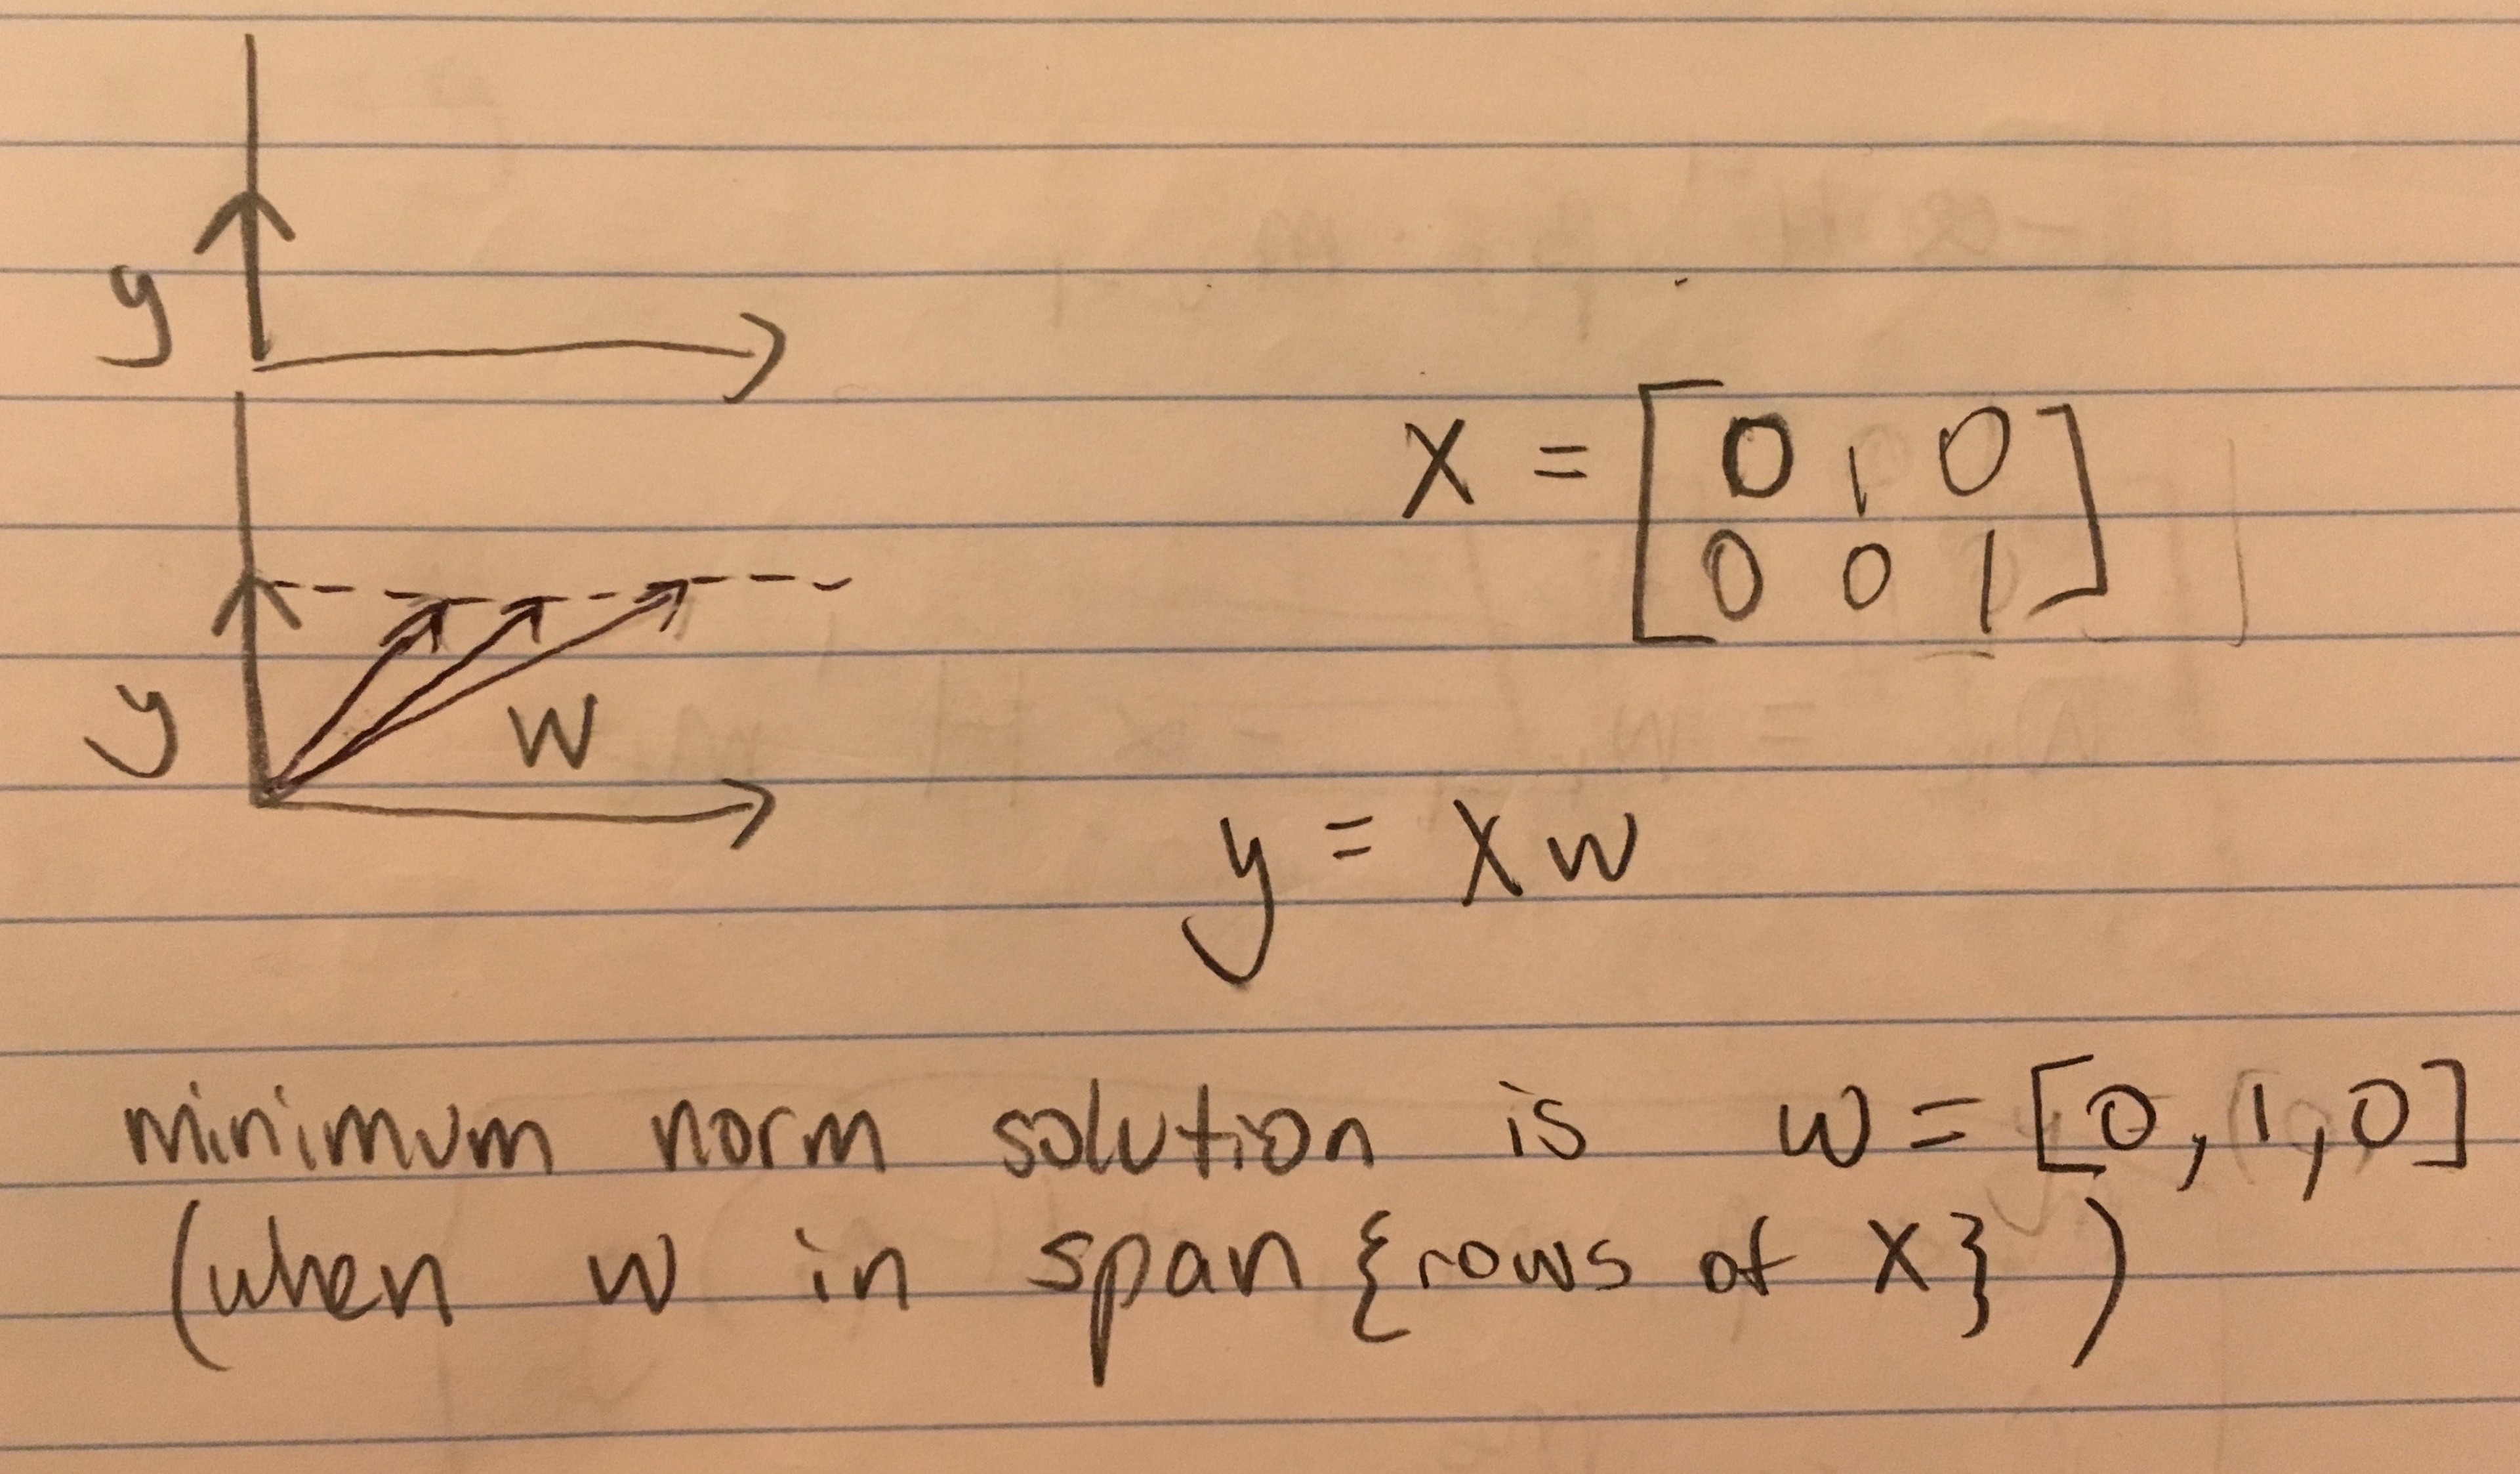
\includegraphics[width=1\textwidth]{min-norm}

\vspace{5mm}
\textbf{Important Idea!} The $w$ with the minimum norm in this case generalizes the best.
%\todo{Maximum margin SVMs}

\newpage

\subsection{Adaptive methods}
\textbf{Claim}:  Suppose $X^T y$ has no components equal to 0, and there exists a scalar $c$ such that $X sign(X^T y) = cy$.

Then when initialized at $w_0 = 0$, AdaGrad, Adam, and RMSProp all converge to the solution $w \propto sign(X^T y)$.

\vspace{3mm}
\textbf{Justification}: 
We want to show for all iterations $k$, 
$$w_k = \lambda_k sign(X^T y)$$

We prove by induction.

\textbf{Base case} We know the assertion holds for $w_0 = 0$, as $\lambda_0 = 0$.

\textbf{Inductive step} Now, given that for some $\lambda_{k-1}$,
$$\nabla R(w_{k-1}) = \lambda_{k-1} sign(X^T y)$$

We can show that for some $\mu_k$, (details in paper)
$$\nabla R(w_k) = \mu_k X^T y$$

The problematic part - what differentiates the adaptive gradient methods - is the $H_k$ term. 
Letting $g_k = \nabla R(w_k)$, then $H_k$ is diagonal matrix such that
$$H_k = \text{diag} \bigg\{ \sqrt{ g_k^2 } \bigg\} = \text{diag} \bigg\{ \sqrt{ \mu_k } |X^T y| \bigg\} =: v_k \text{diag} (  | X^T y | ) $$

$$w_{k+1} = w_k - \alpha_k H_k^{-1} \tilde{ \nabla } f ( w_k + \gamma_k (w_k - w_{k-1})) + \beta_k H_k^{-1} H_{k-1} (w_k - w_{k-1}) $$
$$= \lambda_k \text{sign} (X^T y) - $$
$$\alpha_k {( v_k  | X^T y | )}^{-1}\mu_k X^T y + $$
$$\beta_k {( v_k | X^T y | )}^{-1} v_{k-1} | X^T y | ( \lambda_k - \lambda_{k-1} ) \text{sign} (X^T y)$$
$$= \bigg\{ \lambda_k - \frac{ \alpha_k \mu_k }{ v_k } + \frac{ \beta_k v_{k-1} }{ v_k } ( \lambda_k - \lambda_{k-1} ) \bigg\} \text{sign} (X^T y)$$

\newpage
\subsection{Adaptivity Can Overfit}

\subsubsection{Problem Setting}
Infinite dimensional, $n$ examples. Labels $y^{(i)} \in \{-1, 1\}$, assigned $1$ with probability $p > \frac{1}{2}$.

\begin{equation}
  \begin{split}
   x^{(i)}_j &=
    \begin{dcases}
      y^{(i)},& j = 1, \\
      1, & j = 2, 3, \\
      1, & j = 4 + 5(i - 1), 4 + 5(i - 1) + 1, ..., 4 + 5(i - 1) + 2(1-y^{(i)}) \\
      0, & \text{otherwise}
    \end{dcases}\\
  \end{split}
\end{equation}

\begin{itemize}
	\item Only the first feature is useful (class label)
	\item Next two features are always 1
	\item All other features are unique for each $n$
		\subitem If there label is 1, 1 unique features
		\subitem If there label is -1, 5 unique features
\end{itemize}

\subsubsection{SGD Solution}

SGD will find minimum norm solution --> no generalization problem.

Let $P$ and $N$ by the set of positive and negative examples respectively. 
$\alpha_+$ and $\alpha_-$ are non-negative constants (can be solved for in closed form; see paper).

$$w^{sgd} = \sum_{i \in P} \alpha_+ x_i - \sum_{j \in N} \alpha_- x_j$$

\subsubsection{AdaGrad Solution}

$$u = X^T y = w$$
$$b = \sum_{i=1}^n y^{(-i)}$$

\begin{equation}
  \begin{split}
   u_j &=
    \begin{dcases}
      n,& j = 1, \\
      b, & j = 2, 3, \\
      y_j, & \text{if } j > 3 \text{ and } x_j = 1 \\
      0, & \text{otherwise}
    \end{dcases}\\
  \end{split}
\end{equation}

\begin{comment}
\begin{equation}
  \begin{split}
   \text{sign} (u_j) &=
    \begin{dcases}
      1,& j = 1, \\
      1, & j = 2, 3, \\
      y_j, & \text{if } j > 3 \text{ and } x_j = 1 \\
      0, & \text{otherwise}
    \end{dcases}\\
  \end{split}
\end{equation}
\end{comment}

Satisfies conditions of lemma since $< u, x_i > = y_i + 2 + y_i(3 - 2y_i) = 4y_i$; so
$$w^{ada} \propto \text{sign} (u)$$
So all components of $w^{ada}$ either zero or $\pm \tau$ for some constant $\tau$.

For a new point though, $x^{test}$, the only features that are nonzero for both $x^{test}$ and $w^{ada}$ are the first three.
Thus, the solution will label all unseen data as being in the positive class:
$$< w^{ada}, x^{test} > = \tau ( y^{test} + 2 ) > 0$$

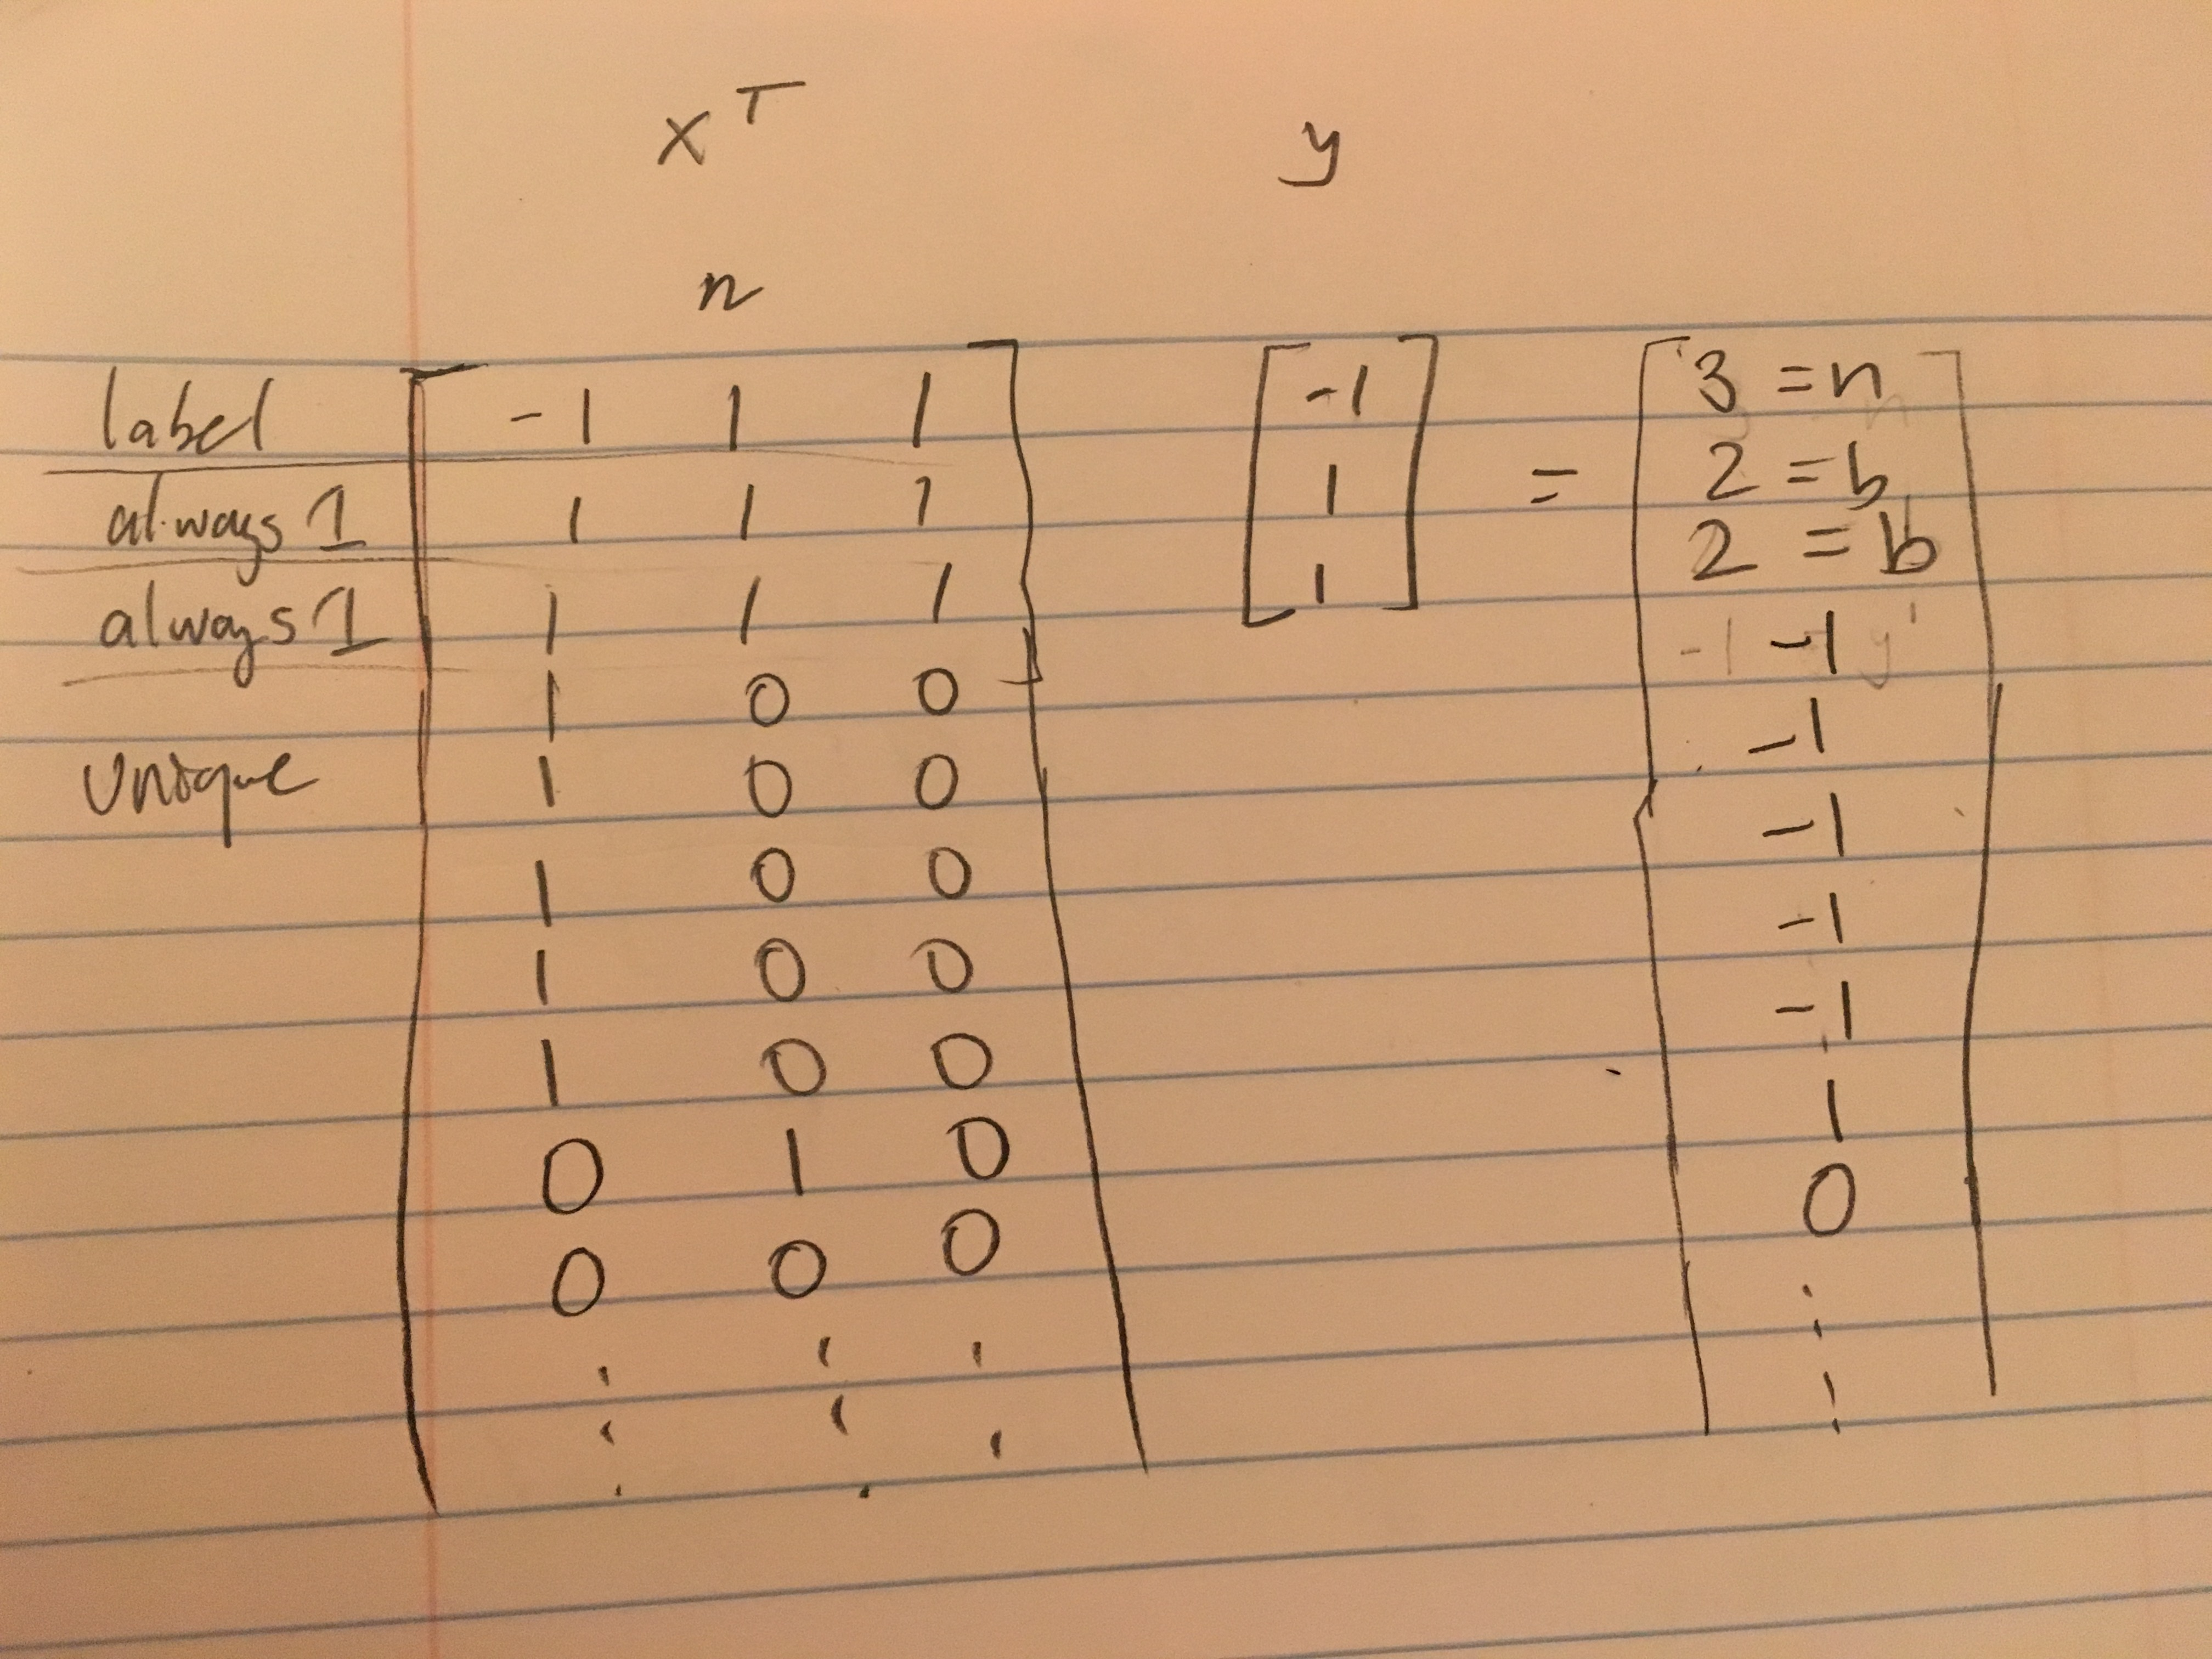
\includegraphics[width=1\textwidth]{infinite}




\newpage
%%%%%%%%%%%%%%%%%%%%%%%%%%%%%%%%%%%%%%%%%%%%%

\section{Empirical Investigations}

\subsection{Methodology}
Strategy: Hold the model, the training objective, and epoch training budget constant, varying only the optimization strategy and measure the generalization error; 5 runs each.

\subsubsection{Learning Rate Tuning}
\begin{itemize}
	\item Initial learning rate: grid search on log scale
	\item LR decay schedule: development-based decay, fixed frequency decay
\end{itemize}

\subsubsection{Training Objective and Models}
\begin{itemize}
	\item CIFAR10
		\subitem VGG+BN+Dropout
		\subitem SGD: $7.65 \pm 0.14\%$ test error
		\subitem RMSProp: $9.60 \pm 0.19\%$ test error
	\item Character-Level Language Model on War and Peace
		\subitem LSTM model
		\subitem SGD: $1.212 \pm 0.001$ test loss
		\subitem RMSProp: test loss very close to SGD's
	\item Constituency Parsing
\end{itemize}

Often adaptive gradient methods outperform SGD early on in training, but their test error of AdaGrad's rate of improvement flatlines earliest.

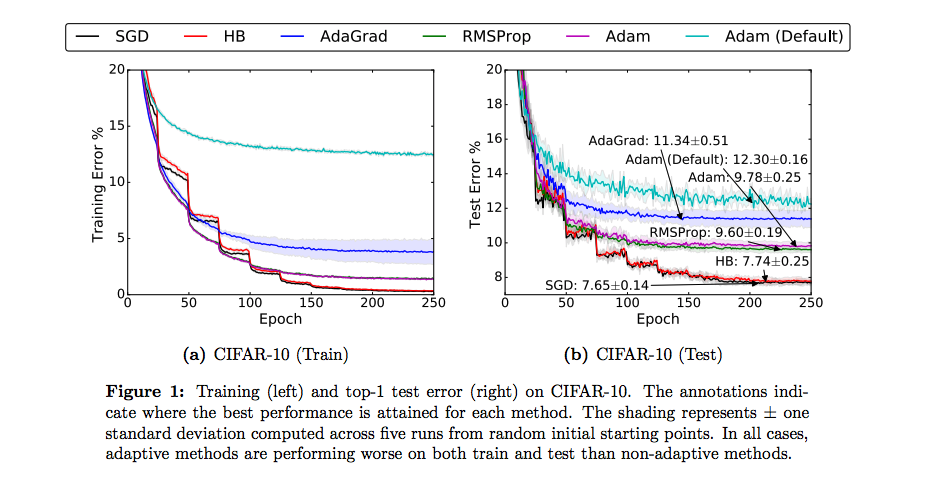
\includegraphics[width=1\textwidth]{generalization-curves}
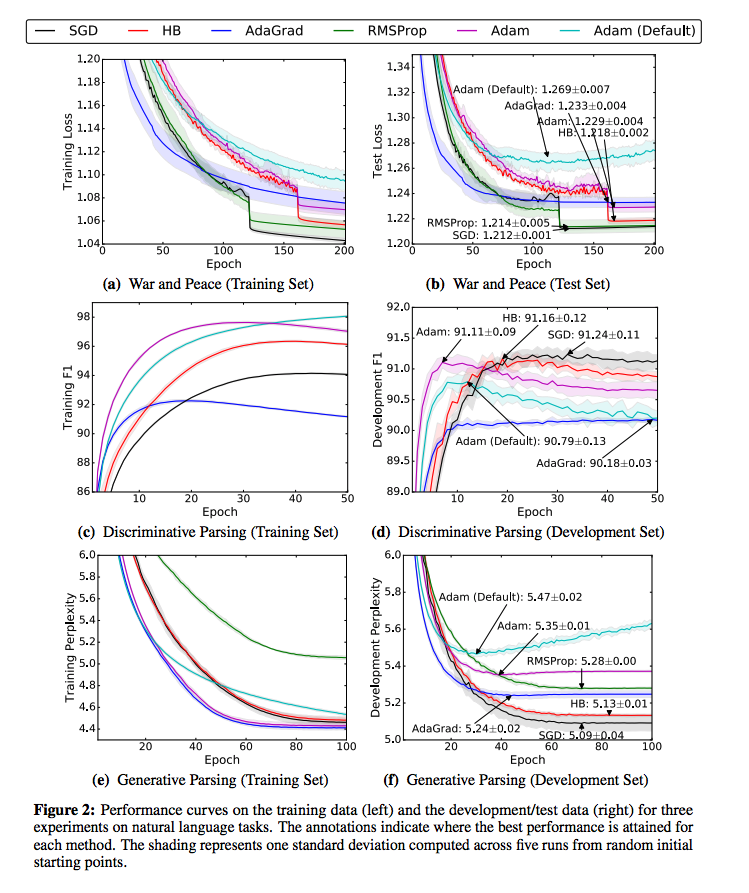
\includegraphics[width=1\textwidth]{curves}

\newpage
%%%%%%%%%%%%%%%%%%%%%%%%%%%%%%%%%%%%%%%%%%%%%
\section{Take-Aways}

\begin{itemize}
	\item In over-parameterized settings, using adaptive gradient methods can give undue influence to spurious features and lead to minima that lead to worse generalization.
	\item Jury is out on whether adaptive gradient methods are beneficial for training GANs.
	\item The difference in generalization (empirically) using SGD vs. Adaptive gradient methods is kind of small, but significant.
	\item Exploring what generalization and regularization in the context of deep learning and over-parameterized settings is very interesting.
\end{itemize}

\bibliographystyle{alpha}
\bibliography{sample}

\end{document}